\documentclass[compress]{beamer}

\mode<presentation>
{
\useoutertheme[subsection=false,footline=authorinstitutetitle]{miniframes}
\useinnertheme{rectangles}
\usecolortheme{whale}
\usecolortheme{orchid}
\usefonttheme{professionalfonts}

\setbeamertemplate{footline}
{
	\begin{beamercolorbox}[wd=0.33\textwidth,ht=2.2ex,dp=0.8ex,leftskip=1.4em,rightskip=1.4em]{author in head/foot}% 
		\usebeamerfont{author in head/foot}%
		\insertshortauthor%
	\end{beamercolorbox}%
 	\vspace*{-3.0ex}\hspace*{0.33\textwidth}%
 	\begin{beamercolorbox}[wd=0.33\textwidth,ht=2.2ex,dp=0.8ex,left,leftskip=1.4em,rightskip=1.4em]{author in head/foot}% 
     	\usebeamerfont{institute in head/foot}%
 		\insertshortinstitute%
 	\end{beamercolorbox}%
  	\begin{beamercolorbox}[wd=0.34\textwidth,ht=2.2ex,dp=0.8ex,left,leftskip=1.4em,rightskip=1.4em]{title in head/foot}
      	\usebeamerfont{title in head/foot}
  		\insertshorttitle
  		\hfill\insertframenumber\,/\,\inserttotalframenumber
  	\end{beamercolorbox}
}

\beamertemplatenavigationsymbolsempty
\setbeamercovered{transparent}

}


\usepackage[ngerman]{babel}
\usepackage[utf8]{inputenc}

% font definitions, try \usepackage{ae} instead of the following
% three lines if you don't like this look
\usepackage{mathpazo}
\usepackage[scaled=.90]{helvet}
%\usepackage{helvet}
\usepackage{courier}
\usepackage{graphics}
\usepackage{amsmath}
\usepackage{amsfonts}
\usepackage{amssymb}


\usepackage[T1]{fontenc}
\usepackage{multicol}
\usepackage{verbatim}
\usepackage{listings}
\usepackage{xcolor}

\newcommand{\textqt}[1]{\frqq #1\flqq\ }


\hypersetup{
   pdftitle={Seminarvortrag},
   colorlinks=false,
   linkcolor=black,
   pdfpagemode=None,
   pdfstartview=Fit
  }

\author[Johannes Pfann]{%
  Johannes Pfann
}


\date{25.05.2016}

\institute[FAU Erlangen-Nürnberg]{
  Lehrstuhl für Software Engineering\\
  Friedrich-Alexander-Universität Erlangen-Nürnberg
}

\subject{Seminar Design Patterns und Anti-Patterns}
\title{Verhaltensmuster: Observer, Command und Visitor}

\newcommand{\changefont}[3]{
\fontfamily{#1}\fontseries{#2}\fontshape{#3}\selectfont}

\lstnewenvironment{beispiel}[3]{
    \lstset{language=#1, 
    numberbychapter=true,
    basicstyle=\ttfamily\small, 
    identifierstyle=\color{black}, 
    keywordstyle=\color{blue}, 
    stringstyle=\color{verde}, 
    commentstyle=\color{red}, 
   	breaklines=true, 
   	numbers=left,
   	label=#2,
   	caption=#3,
   	numberstyle=\small, 
   	frame=single}
   	\begingroup
   	\nopagebreak
   	}
   	{\endgroup}%  	   
   	

%%%%%% Farben 
\definecolor{hellgrau}{rgb}{0.95,0.95,0.95}
\definecolor{dunkelgrau}{rgb}{0.8,0.8,0.8}
%\AtBeginSection[]
%{
%  \begin{frame}
%    \frametitle{Gliederung}
%    \tableofcontents[currentsection, hideothersubsections]
%  \end{frame}
%}

\AtBeginSection[]
{
  \begin{frame}
    \frametitle{Gliederung}
    \tableofcontents[currentsection, hideallsubsections]
  \end{frame}
}

\definecolor{dkgreen}{rgb}{0,0.6,0}
\definecolor{gray}{rgb}{0.5,0.5,0.5}
\definecolor{mauve}{rgb}{0.58,0,0.82}

\usepackage[section]{minted}
\definecolor{mintedbackground}{rgb}{0.95,0.95,0.95}

\newmintedfile[javacode]{java}{
	bgcolor=mintedbackground,
	linenos=true,
	numberblanklines=true,
	numbersep=5pt,
	gobble=0,
	funcnamehighlighting=true,
	tabsize=4,
	obeytabs=false,
	mathescape=false
	samepage=true,
	showspaces=false,
	showtabs =false,
	texcl=false,
	breaklines=true,
	fontsize=\scriptsize,
	style=trac
}


\begin{document}


\frame{\titlepage} 

\begin{frame}
	\frametitle{Gliederung}
	\tableofcontents[hideallsubsections]
\end{frame}


\section[Verhaltensmuster]{Verhaltensmuster}
\subsection{Erzeugungsmuster - Was ist das?}
\begin{frame}
	\frametitle{Erzeugungsmuster -- Was ist das?}
	\begin{block}{Erzeugungsmuster ...}
	\begin{itemize}
		\item klassifizieren die Erzeugung von Objekten
		\item kapseln die konkreten Klassen eines Systems
		\item verbergen konkrete Erzeugungsprozesse dieser Klassen	
	\end{itemize}
	\end{block}	
	\begin{block}{Konsequenzen}
	\begin{itemize}
		\item Erhöhte Flexibilität \textit{wer wann was wie} erzeugt.
		\item System wird unabhängiger von der Zusammenstellung und Erzeugung der verwendeten Objekte
		\item Es wird lediglich mit den abstrakten Schnittstellen gearbeitet
	\end{itemize}
	\end{block}	
\end{frame}

\subsection{Typen von Erzeugungsmustern}
\begin{frame}
	\frametitle{Typen von Erzeugungsmustern}
	\begin{block}{Klassenbasiert}
		Bei klassenbasierten Mustern wird Vererbung verwendet
		\begin{itemize}
			\item Factory Method
		\end{itemize} 	
	\end{block}

	\begin{block}{Objektbasiert}
		Bei objektbasierten Mustern wird der Erzeugungsprozess an andere Objekte delegiert
				\begin{itemize}
					\item \alert<2-> {Singleton}
					\item \alert<2-> {Prototype}
					\item \alert<2-> {Abstract Factory}
					\item Builder				
				\end{itemize}	
	\end{block}
\end{frame}

\section[Observer]{Observer}
\subsection{Definition}
\begin{frame}
  \frametitle{Definition}

  \begin{block}{Zweck}
  	Definition einer 1-zu-n-Abhängigkeit zwischen Objekten, damit im Fall einer Zustandsänderung eines Objekts alle davon abhängigen Objekte entsprechend benachrichtigt und automatisch aktualisiert werden.
  \end{block}
  
\end{frame}

\subsection{Klassendiagramm - Observer Pattern}

\begin{frame}
\frametitle{Klassendiagramm}
\begin{columns} 
    	\column[c]{.35\textwidth} 
    		\begin{itemize}
    			\item 1-zu-n-Abhänigkeit
    			\item Subject benachrichtig Observer
    			\item Zustandsänderung ist Auslöser
    			\item Clients aktualisieren sich selbst
    		\end{itemize}
    	\column[c]{.65\textwidth} 
    			\begin{figure}
					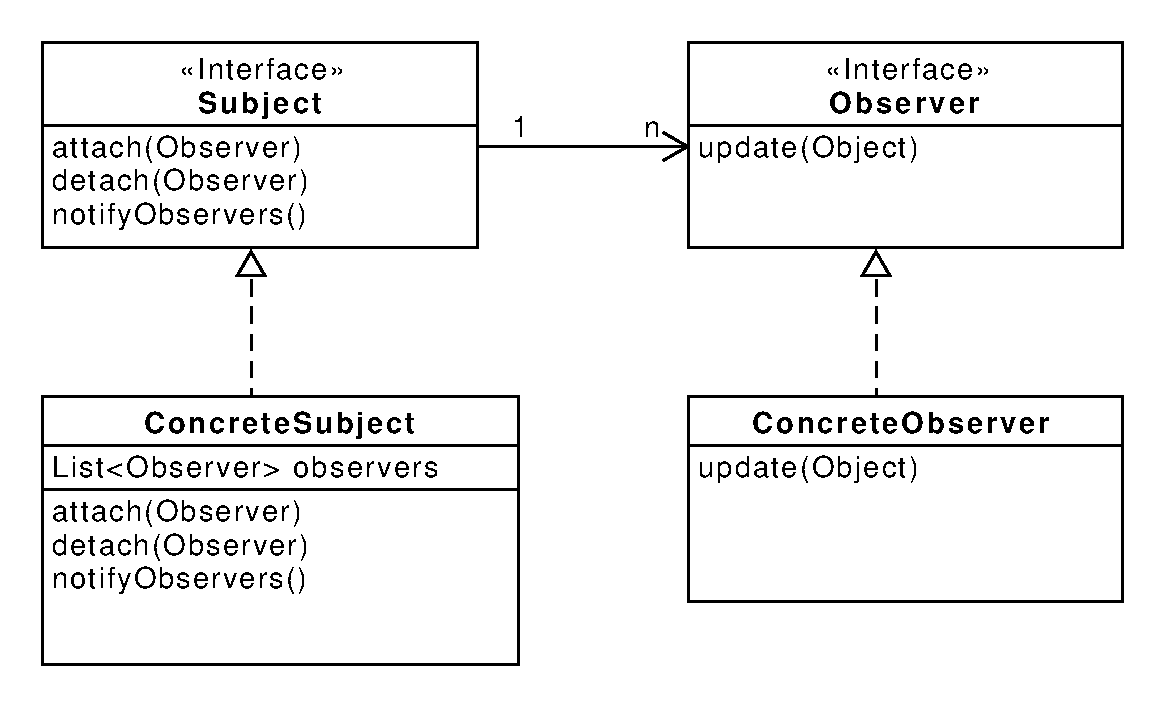
\includegraphics[scale=.37]{paper/observer/observer}
				\end{figure}
  	\end{columns} 
\end{frame}

\subsection{Beispiel - Jobcenter}
\begin{frame}
	\frametitle{Beispiel}
	\begin{itemize}
		\item 1-zu-n-Kommunikation zwischen Jobcenter und Client 
		\item Jobcenter kennt weder Anzahl noch konkrete Clients
		\item Clients bearbeiten ihre Benachrichtigung unterschiedlich
	\end{itemize}		 
  	\begin{figure}
		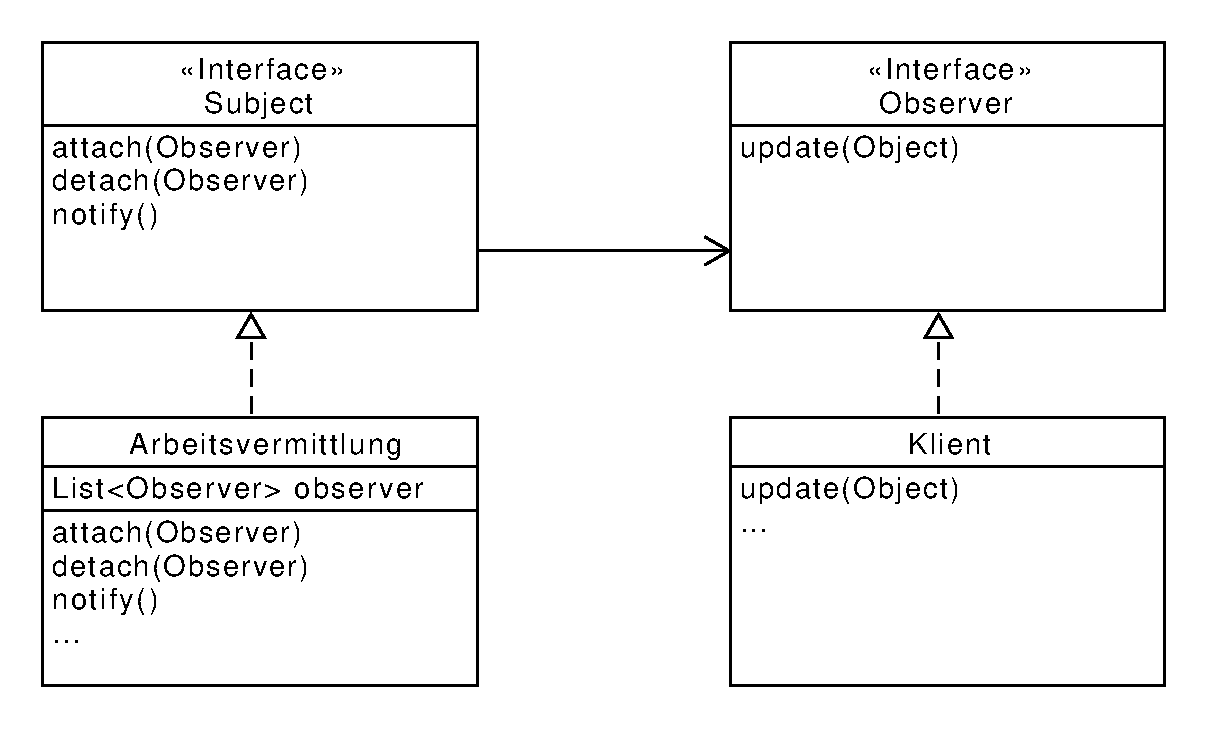
\includegraphics[scale=.4]{paper/observer/arbeitsvermittlung}
	\end{figure}
\end{frame}


\begin{frame}
\frametitle{Beispiel}

		\javacode{resources/observer_Subject_Interface.java} 
		\javacode{resources/observer_Arbeitsvermittlung.java}	  
\end{frame}

\begin{frame}
\frametitle{Beispiel}
		\javacode{resources/observer_Observer_Interface.java}
  		\javacode{resources/observer_Klient.java}	 
\end{frame}

\begin{frame}
	\frametitle{Beispiel}
	\begin{itemize}
		\item Anmeldung der Instanzen aHomepage und aMonitor am aJobCenter 
		\item Speicherung erfolgt in einer Collection<Observer>
		\item Bei einer Zustandsänderung wird die notifyObserver-Methode aufgerufen
		\item Benachrichtigung aller angemeldeten Observer
	\end{itemize}		 
  	\begin{figure}
		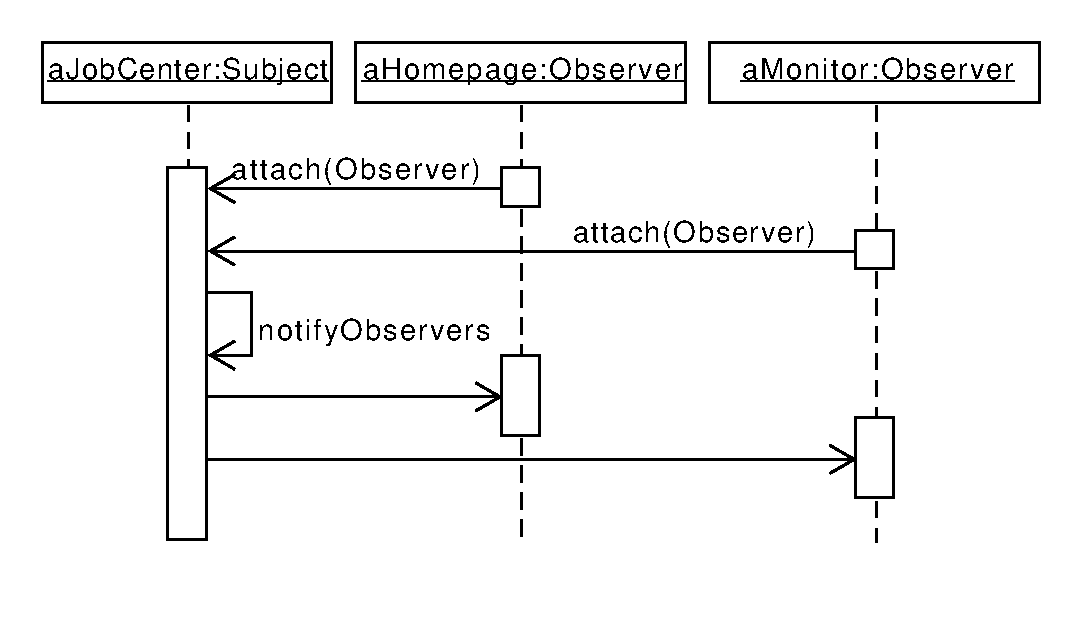
\includegraphics[scale=.4]{paper/observer/observer_sequenz}
	\end{figure}
\end{frame}


\subsection{Implementierungsmöglichkeiten}
\begin{frame}
\frametitle{Implementierungsmöglichkeiten}
		\begin{block}{Push Modell}
		  \begin{itemize}
		  	\item Subject übergibt detaillierte Informationen 
		  	\item Observer hat keinen Zugriff auf Subject
		  	\item Subjekt muss Interesse der Observer kennen
		  \end{itemize}
  		\end{block}
  		\begin{block}{Pull Modell}
  		 \begin{itemize}
		  	\item Subject informiert nur auf Veränderung und übergibt keine Daten
		  	\item Observer muss sich Daten vom Subject holen
		  	\item Observer müssen Subject kennen
		  \end{itemize}  
  		\end{block}
  		Beides kann auch gemischt werden!
\end{frame}

\begin{frame}
\frametitle{Implementierungsmöglichkeiten}
		\begin{block}{Ausführung der Benachrichtigungsmethode durch Subject}
  		 \begin{itemize}
  		 	\item z.B. in Add-Methoden
		  	\item Weniger fehleranfällig
		  	\item Jedoch zu häufige Updates
		  \end{itemize}  
  		\end{block}		
  		\begin{block}{Ausführung der Benachrichtigungsmethode von Extern}
		  \begin{itemize}
		  	\item Fehleranfälliger
		  	\item Regulierung der Updates
		  \end{itemize}
  		\end{block}	
\end{frame}

\begin{frame}
\frametitle{Implementierungsmöglichkeiten}
		  \begin{block}{Observer beobachten mehrere Subjects}
		  	\begin{itemize}
		  		\item Observer registriert sich bei mehreren Subjects
		  		\item Muss allerdings unterschiedlich darauf reagieren
		  		\item Lösung: Erweiterung der update-Methode mit Subject
		  	\end{itemize}
		  \end{block}
		\javacode{resources/observer_erweiterung_update.java}  		
\end{frame}

\begin{frame}
\frametitle{Implementierungsmöglichkeiten}
		\begin{block}{Observer gibt sein Interesse an}
  		 \begin{itemize}
		  	\item Observer registrieren sich für ein bestimmtes Event
		  	\item Subject kümmert sich um die Zuordnung
		  	\item Benachrichtigung wird effizienter
		  	\item Subject wird komplexer
		  \end{itemize}  
  		\end{block}		
  		\javacode{resources/observer_sortToObserverlist.java}  
\end{frame}

\begin{frame}
\frametitle{Implementierungsmöglichkeiten}
		\begin{block}{Einführung eines \texttt{ChangeManager}}
  		 \begin{itemize}
		  	\item Subject delegiert Aufgaben zu ChangeManager
		  	\item ChangeManger hat drei Aufgaben:
		  	\begin{itemize}
		  		\item Legt Zuordnung von Subject, Observer und Demand fest
		  		\item Legt Aktualisierungsstrategie fest
		  		\item Führt die Aktualisierung aus
		  	\end{itemize}
		  \end{itemize}  
  		\end{block}		
  		\begin{figure}
		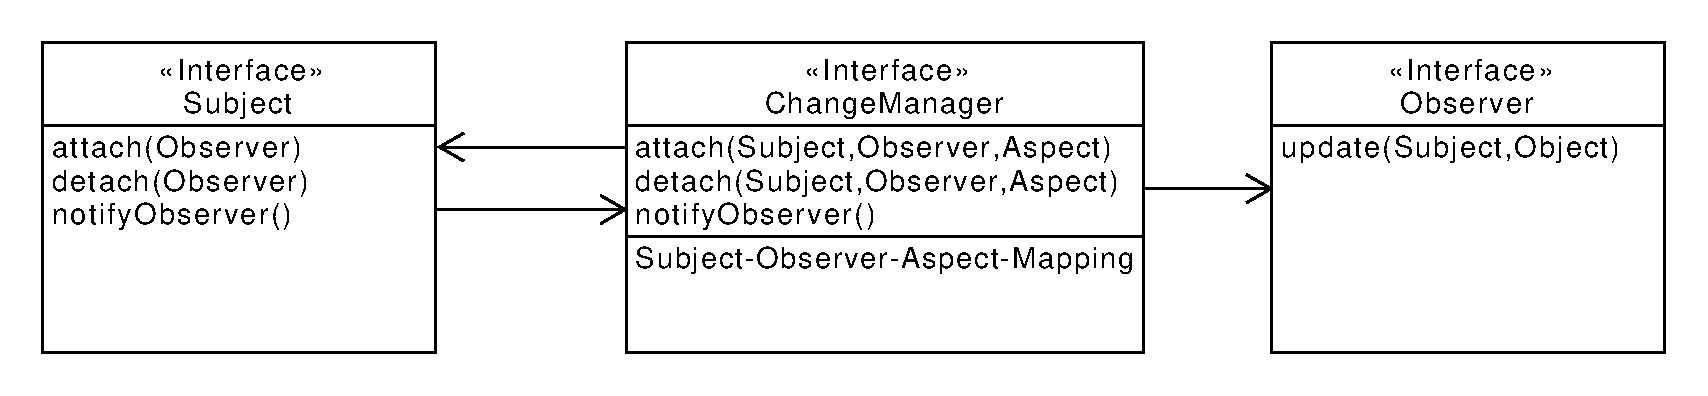
\includegraphics[scale=.4]{paper/observer/changemanager}
	\end{figure}
\end{frame}

%\begin{frame}
%\frametitle{Observer-Pattern als Fehlerquelle}
%		\begin{block}{Konsistenz vor dem Update}
%			\begin{itemize}
%  				\item Vorsicht bei Vererbung
%  			\end{itemize}  
%  		\end{block}		
%	\begin{block}{Verwaiste Referenzen auf gelöschte Subjects}
%			\begin{itemize}
%  				\item Subject wird gelöscht und Observer wissen nichts darüber
%  			\end{itemize}  
%  		\end{block}	
%  		\begin{block}{Komplexe Strukturn}
%			\begin{itemize}
%  				\item Zyklische Abhängigkeiten
%  				\item Komplexe Fehlersuche
%  			\end{itemize}  
%  		\end{block}			
%\end{frame}


\subsection{Fazit}
\begin{frame}
	\frametitle{Fazit}
	\begin{columns} 
    	\column[t]{.50\textwidth} 
    		\begin{exampleblock}{Vorteile}
    			\begin{itemize}
    				\item Lose Kopplung
    				\item Flexibilität
    				\item Automatische Benachrichtigung
    			\end{itemize}
    		\end{exampleblock}
    	\column[t]{.50\textwidth} 
    		\begin{alertblock}{Nachteile}
    			\begin{itemize}
    				\item Komplexität
    				\item Gefahr von Zyklen
    			\end{itemize}
    		\end{alertblock}
  	\end{columns}   	  		
\end{frame}

\section[Command]{Command}
\subsection{Definition}
\begin{frame}
  \frametitle{Definition}
  \begin{block}{Zweck}
  	Kapselung eines Requests als Objekt, um so die Parametrisierung von Clients mit verschiedenen Requests zu ermöglichen.
  \end{block}
  
\end{frame}

\subsection{Klassendiagramm - Command Pattern}
\begin{frame}
	\frametitle{Klassendiagramm}		
	\begin{itemize}
		\item Kapselt Request in ein eigenes Command-Object
		\item Implementierung von Command kennt den Empfänger
	\end{itemize}	
  	\begin{figure}
		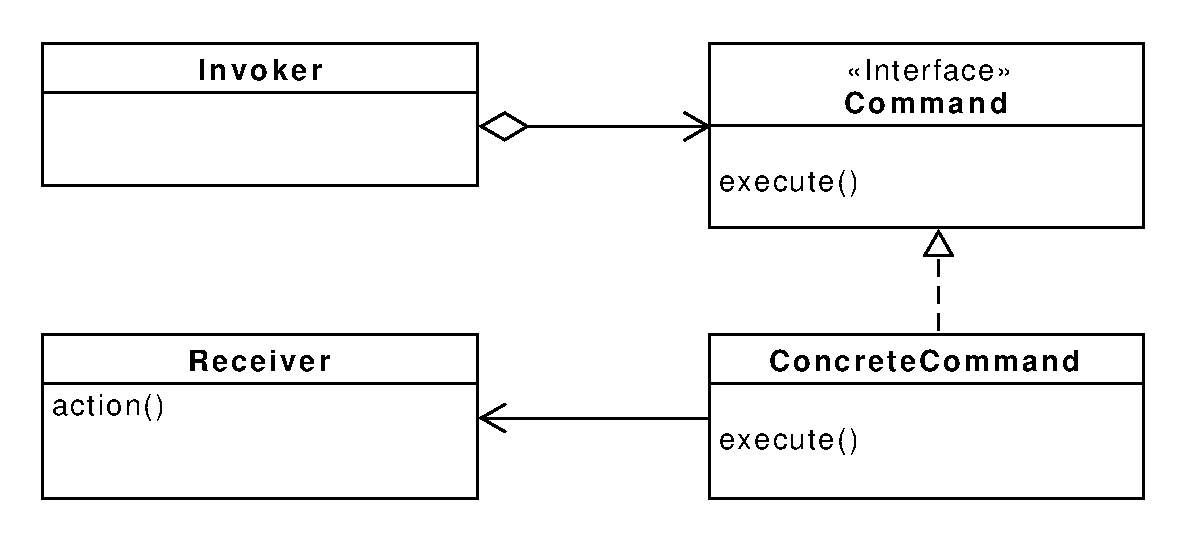
\includegraphics[scale=.4]{paper/command/command}
	\end{figure}
\end{frame}

\subsection{Beispiel - Deliver Service}
\begin{frame}
	\frametitle{Beispiel}
	\begin{itemize}
		\item Verschiedene Objekte die unterschiedlich ausgeliefert werden müssen
		\item Unterschiedliche Kunden
	\end{itemize}	
	
  	\begin{figure}
		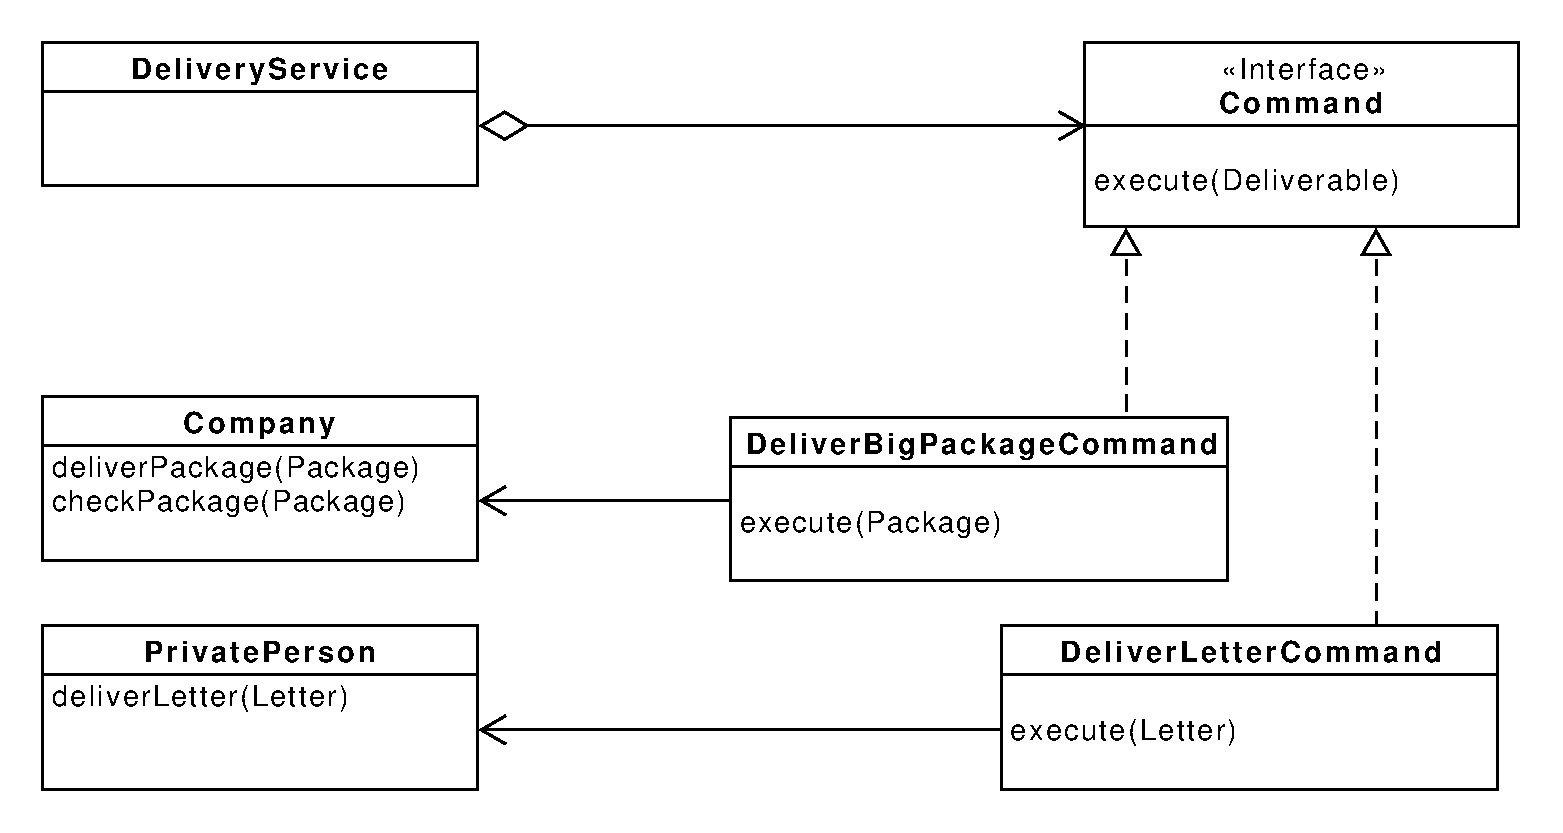
\includegraphics[scale=.4]{paper/command/DeliverService}
	\end{figure}
\end{frame}


\begin{frame}
	\frametitle{Beispiel}
  	\begin{figure}
		\javacode{resources/command_interface.java} 
		\javacode{resources/command_DeliverBigPackageCommand.java} 
	\end{figure}
\end{frame}

\begin{frame}
	\frametitle{Beispiel}
  	\begin{figure}
		\javacode{resources/command_DeliveryService.java} 
		\javacode{resources/command_main.java}
	\end{figure}
\end{frame}

\subsection{Implementierung}

\begin{frame}
	\frametitle{Implementierungsmöglichkeiten}
  	\begin{block}{Undo-Funktion}
\begin{itemize}
		\item Erweiterung des Interfaces Command mit undo-Methode
		\item Der Invoker kann sich Commands merken und auf diese eine undo-Methode aufrufen
		\item das ConcreteCommand muss dann ggf. Daten speichern:
			\begin{itemize}
				\item Receiver-Objekt
				\item Die Argumente, die für die Ausführung angewendet wurden
				\item Alle relevanten Orginalwerte im Receiver-Objekt
			\end{itemize}
	\end{itemize}	
   \end{block}
\end{frame}

\begin{frame}
	\frametitle{Implementierungsmöglichkeiten}
  	\begin{block}{Makro-Befehle}
		\begin{itemize}
			\item Mehrere Receiver könnten gleichzeitig durch ein Command bearbeitet werden
		\end{itemize}	
   \end{block}
   \javacode{resources/command_macro_command.java}
\end{frame}



\begin{frame}
	\frametitle{Implementierungsmöglichkeiten}
  	\begin{block}{Intelligenz der Commandobjekte}
		\begin{itemize}
		\item Command übernimmt vollständig die Logik
		\item Comnand delegiert die komplette Logik an den Receiver
	\end{itemize}	
   \end{block}
   
		\javacode{resources/command_command_logic.java}
		\javacode{resources/command_deligate_logic.java}
		
\end{frame}


\subsection{Fazit}
\begin{frame}
	\frametitle{Fazit}
	\begin{columns} 
    	\column[t]{.50\textwidth} 
    		\begin{exampleblock}{Vorteile}
    			\begin{itemize}
    				\item Entkopplung von Befehl und Ausführung
    				\item Hohe Flexibilität durch Austauschbarkeit
    			\end{itemize}
    		\end{exampleblock}
    	\column[t]{.50\textwidth} 
    		\begin{alertblock}{Nachteile}
    			\begin{itemize}
    				\item Hohe Anzahl von Klassen
    			\end{itemize}
    		\end{alertblock}
  	\end{columns}   	  		
\end{frame}

\section[Visitor]{Visitor}
\subsection{Definition}
\begin{frame}
  \frametitle{Definition}
  \begin{block}{Zweck}
  	 Das
Design Pattern Visitor ermöglicht die Definition einer neuen Operation, ohne die Klasse der
von ihr bearbeiteten Elemente zu verändern.
  \end{block}
  
\end{frame}

\subsection{Klassendiagramm - Visitor Pattern}
\begin{frame}
	\frametitle{Visitor Pattern}		
	\begin{itemize}
		\item Elemente der Objektstruktur fest
		\item Operationen auf Objektstruktur sollen austauschbar und erweiterbar sein
	\end{itemize}	
  	\begin{figure}
		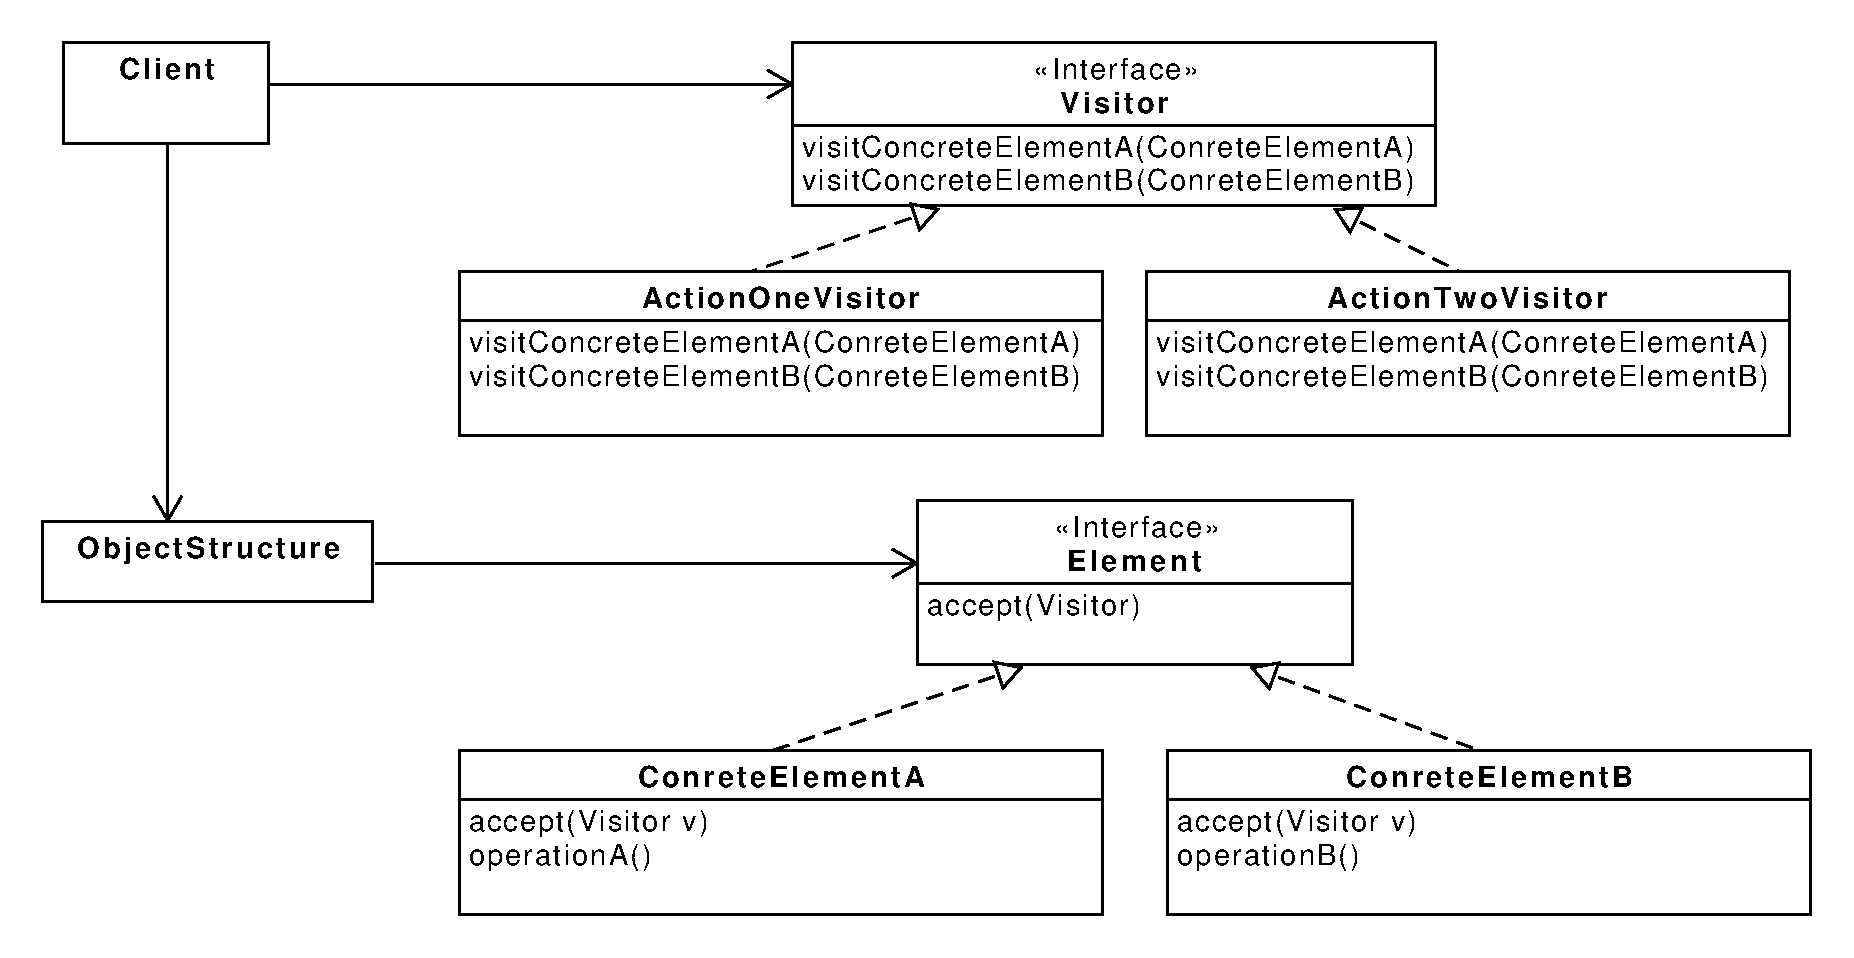
\includegraphics[scale=.3]{paper/visitor/visitor}
	\end{figure}
\end{frame}

\subsection{Beispiel - Kitchen}
\begin{frame}
	\frametitle{Klassendiagramm}
	\begin{itemize}
		\item Die verschiedenen Sorten die wir bearbeiten möchten, bleiben konstant
		\item Wie wir allerdings diese bearbeiten ist noch unklar.
	\end{itemize}	
	
  	\begin{figure}
		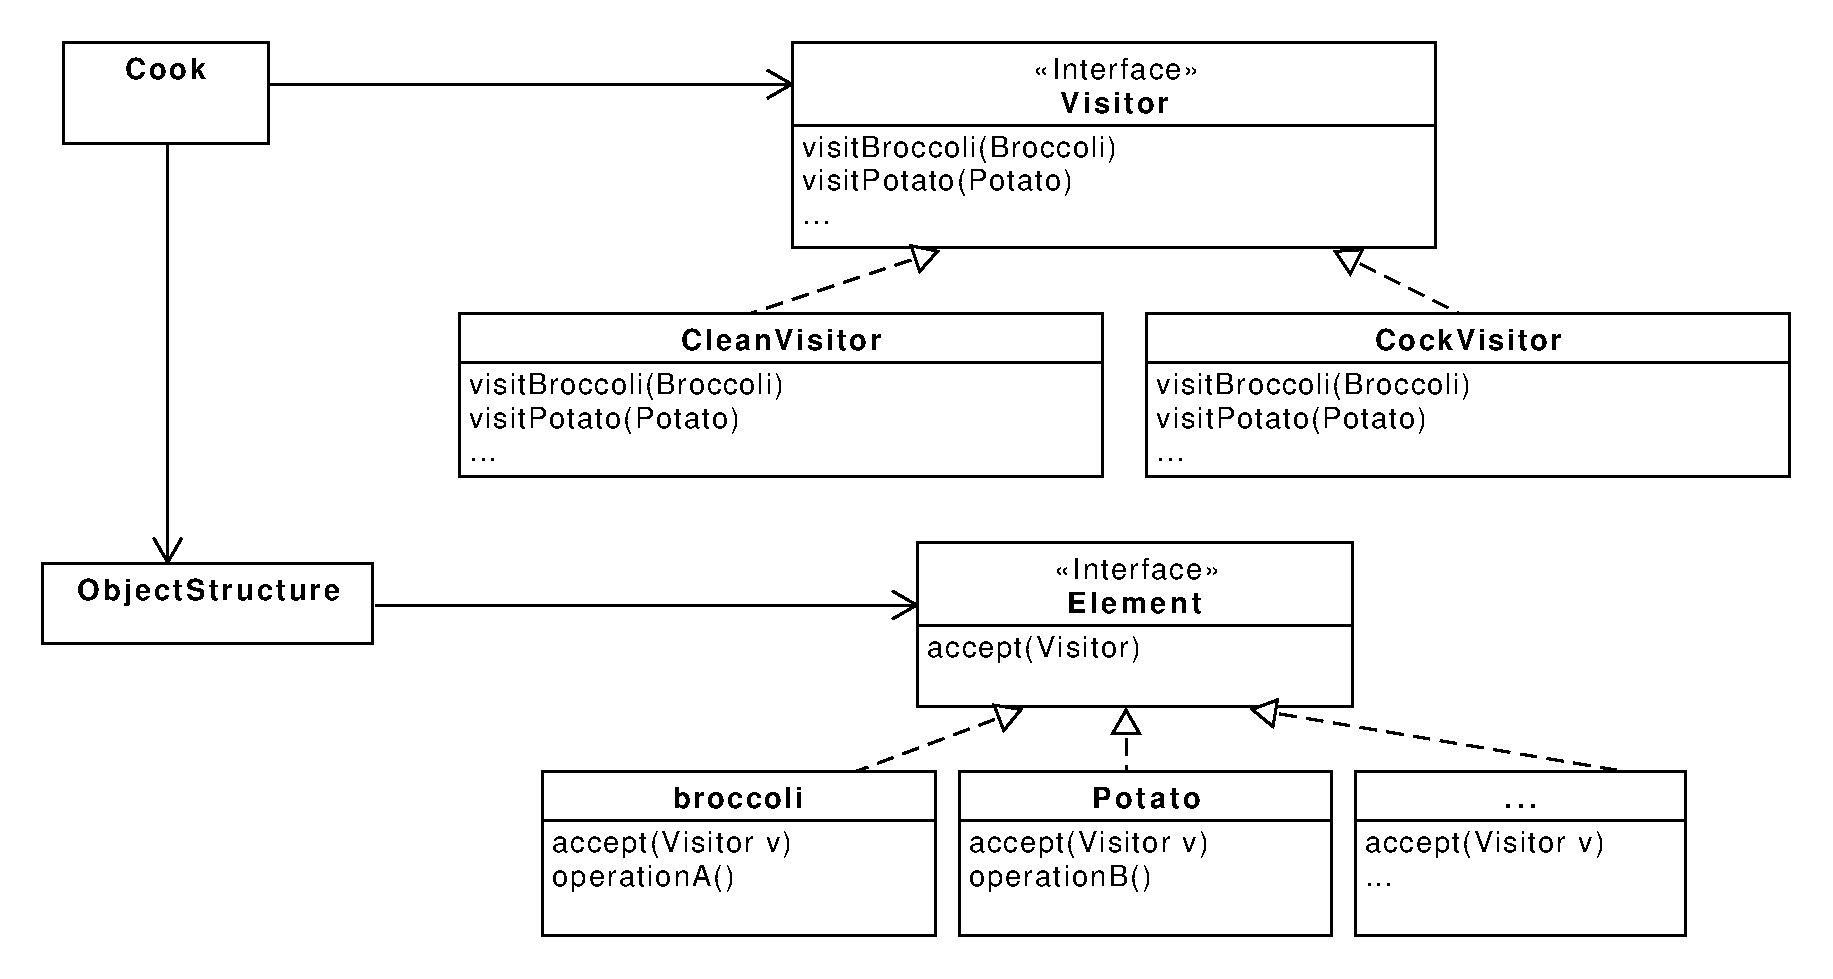
\includegraphics[scale=.3]{paper/visitor/kitchen}
	\end{figure}
\end{frame}



\begin{frame}
	\frametitle{Schnittstellen}
  	\begin{figure}
		\javacode{resources/visitor_element_interface.java} 
		\javacode{resources/visitor_visitor_interface.java}
	\end{figure}
\end{frame}

\begin{frame}
	\frametitle{Implementierungen}
  	\begin{figure}
		\javacode{resources/visitor_potato.java} 
		\javacode{resources/visitor_cleanvisitor.java}
	\end{figure}
\end{frame}

\begin{frame}
	\frametitle{Client}
  	\begin{figure}
		\javacode{resources/visitor_main.java} 
	\end{figure}
\end{frame}

\begin{frame}
	\frametitle{Implementierungen}
  \begin{block}{Wer ist für die Traversierung der Objektstruktur verantwortlich}
  	\begin{itemize}
  		\item In der Objektstuktur
  		\item Im Visitor-Objekt
  		\item In einem eigenen Iterator-Objekt
  	\end{itemize}
  \end{block}
\end{frame}


\begin{frame}
	\frametitle{Implementierung}
  \begin{block}{Objektstruktur}
  	\begin{itemize}
  		\item Objektstruktur kümmert sich um die Traversierung 
  		\item Visitor muss der Objektstruktur übergeben werden
  		\item Realisierbar durch z.B Composide-Pattern
  	\end{itemize}
  \end{block}
  \javacode{resources/visitor_composide_example.java} 
\end{frame}

\begin{frame}
	\frametitle{Implementierung}
  \begin{block}{Iterator}
  	\begin{itemize}
  		\item Zugriff auf Elementen einer Objektstruktur, ohne die  Objektstruktur zu kennen.
  		\item Die Visitor-Objekten den Iterator übergeben
  		\item Beim Zugriff eines Elements die accept-Methode aufrufen

  	\end{itemize}
  \end{block}
	\begin{block}{Im Visitor-Objekt}
  	\begin{itemize}
  		\item Objektstruktur wird den konkreten Visitors übergeben
  		\item Visitor übernimmt jetzt die Traversierung
  		\item Nachteil: Traversierung in jedem Visitor
  		\item Vorteil: Flexibler in der Steuerung für bestimmte Aufgaben

  	\end{itemize}
  \end{block}
\end{frame}


\begin{frame}
	\frametitle{Implementierung}

  \javacode{resources/visitor_trav_visitor_object.java} 
\end{frame}

\subsection{Fazit}
\begin{frame}
	\frametitle{Fazit}
	\begin{columns} 
    	\column[t]{.50\textwidth} 
    		\begin{exampleblock}{Vorteile}
    			\begin{itemize}
    				\item Leicht neue Operationen auf eine Objektstruktur zu implementieren
    				\item Selektives bearbeiten einzelner Elemente einer Objektstruktur
    				\item Flexiblität indem Commands leicht ausgetauscht werden können
    			\end{itemize}
    		\end{exampleblock}
    	\column[t]{.50\textwidth} 
    		\begin{alertblock}{Nachteile}
    			\begin{itemize}
    				\item Enge Kopplung des Visitor mit den Elementen einer Objektstruktur
    				\item Elemente müssen über öffentliche Methoden und Attribute dem Visitor den Zugriff bereitstellen
    			\end{itemize}
    		\end{alertblock}
  	\end{columns}   	  		
\end{frame}


\section[Quellen]{Quellen}
\begin{thebibliography}{5cm}
 \bibitem[1]{1} Gamma, Helm, Johnson, Vlissides: „Design Patterns -
Entwurfsmuster als Elemente wiederverwendbarer
Objektorientierter Software“.
1. Auflage, mitp Verlags GmbH, 2015.
   \bibitem[2]{2} Eilebrecht, Starke: „Patterns Kompakt - Entwurfsmuster für
effektive Software-Entwicklung“.
3. Auflage, Spektrum Verlag, Heidelberg 2010.
   \bibitem[3]{3} Michael Inden: Der Weg zum Java-Profi. 3 Auflage dpunkt.verlag
 \bibitem[4]{4} Eric Freeman, Elisabeth Freeman, Kathy Sierra, Bert Bates: Entwurfsmuster von Kopf bis Fuß. 1 Auflage O'Reilly Media, Inc
\end{thebibliography}



\end{document}

